
%% Version for one sided printing:
% margins: left 40mm, right 25mm, top and bottom 25mm
% (BUT LaTeX adds automaticly 1in)
\documentclass[12pt,a4paper]{report}
\setlength\textwidth{145mm}
\setlength\textheight{247mm}
\setlength\oddsidemargin{15mm}
\setlength\evensidemargin{15mm}
\setlength\topmargin{0mm}
\setlength\headsep{0mm}
\setlength\headheight{0mm}
% \openright makes following text start on right side of book
\let\openright=\clearpage

%% Version for two sided printing:
% \documentclass[12pt,a4paper,twoside,openright]{report}
% \setlength\textwidth{145mm}
% \setlength\textheight{247mm}
% \setlength\oddsidemargin{15mm}
% \setlength\evensidemargin{0mm}
% \setlength\topmargin{0mm}
% \setlength\headsep{0mm}
% \setlength\headheight{0mm}
% \let\openright=\cleardoublepage

%\usepackage[T1]{fontenc}
\usepackage[utf8]{inputenc}
%\usepackage[american]{babel}

\usepackage{comment}
\usepackage{setspace}

\usepackage{graphicx}
%\usepackage{amsthm}
\usepackage{booktabs}


\usepackage[autostyle]{csquotes}
\usepackage{xspace}

\usepackage[
	backend=biber,
	style=alphabetic,
	backref=true,
%	natbib=true,
%	url=false, 
%	doi=true,
%	eprint=false
]{biblatex}
\renewcommand{\labelalphaothers}{*}
\addbibresource{bibliography.bib}

\usepackage{color}
\definecolor{linkClr}{RGB}{127,0,0}  % dark red
\definecolor{citeClr}{RGB}{0,127,0}  % dark green
\definecolor{urlClr}{RGB}{0,0,127}  % dark blue

\usepackage{listings}  % \lstlisting enviroment - source code highliting

\usepackage{lsystemSyntax}  % uses packages color and listings

\usepackage[unicode]{hyperref}  % after all other packages
\hypersetup{
	pdftitle=L-systems online,
	pdfauthor=Marek Fišer,
	pdfkeywords={keyword1} {key2},
	colorlinks=true,
	linkcolor=linkClr,
	citecolor=citeClr,
	urlcolor=urlClr
}

%%% Little tweaks

% These macros remove white space above headers of chapters.
\makeatletter
\def\@makechapterhead#1{
  {\parindent \z@ \raggedright \normalfont
   \Huge\bfseries \thechapter. #1
   \par\nobreak
   \vskip 20\p@
}}
\def\@makeschapterhead#1{
  {\parindent \z@ \raggedright \normalfont
   \Huge\bfseries #1
   \par\nobreak
   \vskip 20\p@
}}
\makeatother

% Definition of chapter macro. Chapters are not numbered but they are in TOC.
\def\chapwithtoc#1{
\chapter*{#1}
\addcontentsline{toc}{chapter}{#1}
}

% default path for graphics
\graphicspath{{img/}}

% macros for L-system to avoid hyphenation of it.
\newcommand{\lsystem}{\mbox{L-system}\xspace}
\newcommand{\lsystems}{\mbox{L-systems}\xspace}

% for carons with t, d
\newcommand{\varcaron}{\hspace{-1.5pt}'\hspace{-1pt}}

\renewcommand{\ttdefault}{pcr}  % to allow bold in tt font

\begin{document}

% A little freer hyphenation settings than the default.
%\lefthyphenmin=2
%\righthyphenmin=2

%
\pagestyle{empty}
\begin{center}

\large

Charles University in Prague

\medskip

Faculty of Mathematics and Physics

\vfill

{\bf\Large BACHELOR THESIS}

\vfill

\centerline{\mbox{
\includegraphics[width=60mm]{logo}}}

\vfill
\vspace{5mm}

{\LARGE Marek Fišer}

\vspace{15mm}

% Name of thesis exactly according to the specification.
{\LARGE\bfseries L-systems online}

\vfill

% Official name of department or institute where the work was officially specified.
% (According to Internal Structure of MFF UK)
Department of Software and Computer Science Education

\vfill

\begin{tabular}{rl}

Supervisor of the bachelor thesis: & RNDr. Josef Pelikán \\
\noalign{\vspace{2mm}}
Study program: & Computer Science \\
\noalign{\vspace{2mm}}
Specialization: & Programming \\
\end{tabular}

\vfill

Prague 2012

\end{center}






































%%% Následuje vevázaný list -- kopie podepsaného "Zadání bakalářské práce".
%%% Toto zadání NENÍ součástí elektronické verze práce, nescanovat.

%
%%% At this point, can be written any thank (head work, literature, etc.)

\openright

\noindent
Dedication.










































%
\vglue 0pt plus 1fill

\noindent
I declare that I carried out this bachelor thesis independently, and only with the cited
sources, literature and other professional sources.

\medskip\noindent
I understand that my work relates to the rights and obligations under the Act No.
121/2000 Coll., the Copyright Act, as amended, in particular the fact that the Charles
University in Prague has the right to conclude a license agreement on the use of this
work as a school work pursuant to Section 60 paragraph 1 of the Copyright Act.

\vspace{10mm}

\hbox{\hbox to 0.5\hsize{%
In ................  date ................
\hss}\hbox to 0.5\hsize{%
signature of the author
\hss}}

\vspace{20mm}









































\chapter*{\lsystems online}

\subsection*{Marek Fišer}

\section*{Abstrakt}

%\begin{otherlanguage*}{czech}
\mbox{L-systém} je v nejjednodušší podobě varianta bezkontextové gramatiky.
Byl vyvi\-nut a používá se hlavně pro modelování růstu rostlin, ale s jeho pomocí se také dají vytvářet obecné fraktály, modely měst nebo dokonce hudba.
Pokud někoho \mbox{L-systémy} zaujmou a chce s nimi experimentovat, je těžké najít aplikaci, která by mu to umožňovala.
Cílem této práce bylo vytvořit online systém pro práci a experimentování s L-systémy pro široké spektrum uživatelů.
Výsledné řešení se skládá ze dvou částí.

První část je univerzální, snadno rozšiřitelná knihovna pro zpracování \mbox{L-sys}\-témů.
Svou rozšiřitelnost dosahuje vysokou modularitou, vstup zpracovává pros\-třednic\-tvím systému propojených komponent, které jsou specializované na kon\-krét\-ní činnost.
To také přispívá k přehlednosti a spolehlivosti celku.
Navíc je knihovna zcela nezávislá a multiplatformní, lze ji tedy použít i v jiných aplikacích.

Druhá část je moderní webové rozhraní, které bylo navrženo tak, aby bylo srozumitelné pro nováčky a zároveň aby nabízelo pokročilé funkce pro nároč\-nější uživatele.
%Pro vizualizaci 3D \mbox{L-systémů} využívá moderní technologie jako HTML5 WebGL.
Součástí webu je i galerie L-systémů, do které může každý uživatel přispívat a tvořit tak komunitu.
Webové rozhraní plně využívá schopnosti navr\-žené knihovny a slouží tak i jako ukázka jejího použití.
%\end{otherlanguage*}































\singlespacing
\openright
\pagestyle{plain}
\setcounter{page}{1}
%\tableofcontents

\onehalfspacing

\chapwithtoc{Introduction}
\label{sec:Introduction}

\lsystem (also called Lindenmayer system) is mathematical formalism developed for plant growth modeling by Aristid Lindenmayer in 1968~\cite{Lin68}.
An example of plant modeled by \lsystem is in \autoref{fig:introLilac}.
In the simplest form an \lsystem is variant of regular or \mbox{context-free} grammar.
By rewriting (deriving) initial string of symbols (also called axiom) with rewrite rules from grammar \lsystem produces string of symbols which can be interpreted in many different ways.
In first \lsystems by Lindenmayer were symbols interpreted as cells of algae.
A different approach was taken by Przemyslaw Prusinkiewicz who interpreted \lsystem symbols with \mbox{Logo-like} turtle\footnote{
	Logo is computer programming language developed for use in education of programming for children.
	Logo controls cybernetic turtle which is drawing on 2D canvas.}~\cite{Pru85}.
With this method he obtained more plant-like structures and fractals~\cite{CD93}.
In \autoref{fig:introHTree} you can see H-tree fractal created by \lsystem.

\begin{figure}[h!]
	\subfloat[Model of lilac panicle]{
		\includegraphics[width=0.49\linewidth]{lilac}
		\label{fig:introLilac}
	} \hfill
	\subfloat[H-tree fractal]{
		
\includegraphics[width=0.49\linewidth]{HTree}
		\label{fig:introHTree}
	}
	\caption{Examples of models created by \lsystem}
\end{figure}


Over the time \lsystems were used in many areas.
For example they were used to generate rivers in fractal mountains~\cite{PH93}, streets in virtual cities~\cite{PM01} and to describe subdivision of curves~\cite{PSSK03}.
\lsystems can be used in other fields than computer graphics for example in music generation~\cite{HCJ99, Man06}.
They are still used in plant modeling.
Plant models generated with \lsystems are used in modern video games or films, for example they were used to generate many plants and trees for the famous film Avatar~\cite{Wor08, Dun10}.~\footnote{\citeauthor{SBM10} presented reverse method -- automatic generation of \lsystems from 2D model~\cite{SBM10}.}

\lsystems has wide variety of interesting applications but it is hard to find some place to experiment with them.
There are two base types of \lsystem generators, web-based and desktop applications.
Web-based \lsystem generators are easily accessible but they are often too primitive and do not offer nothing more than generation of simple fractals (see \autoref{sec:WebBasedGenerators}).
Some of them do not work in the most used browsers.

Desktop applications generally offer more options than web-based but most of them is also quite simple and do not offer advanced types of \lsystems.
There are some complex applications that offer pretty good features but they are expensive, it is not easy to control them or they are old and not maintained (see \autoref{sec:DesktopGenerators}).
The problem with desktop applications is also in compatibility with user's operating system, its version and installed libraries.

The main goal of this work is to take the good from both approaches and create online feature-rich development environment for anybody who wants to experiment with \lsystems.
The development environment will be divided into two parts, web user interface and \lsystem processing library.

\begin{wrapfigure}{r}{0.5\textwidth}%
	\vspace{6pt}%
	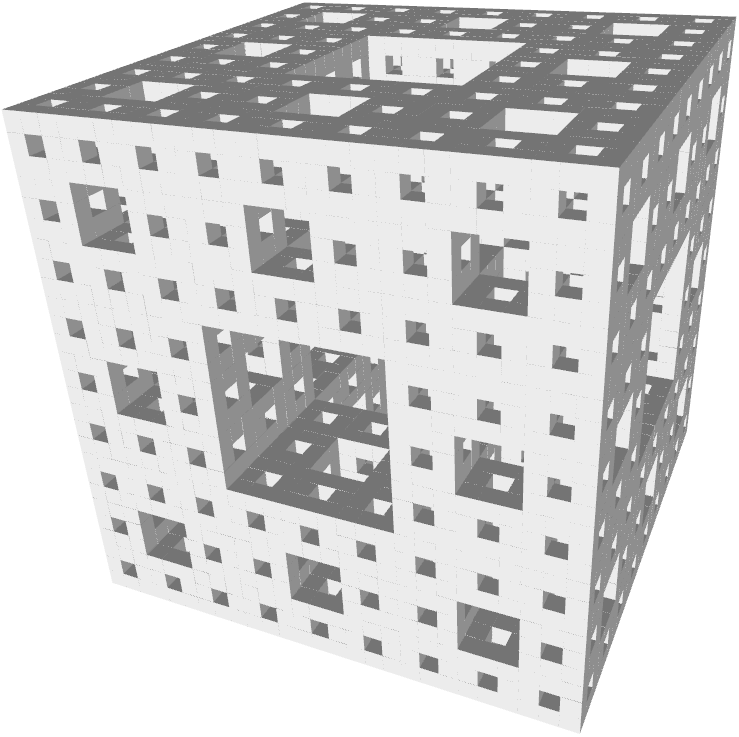
\includegraphics[width=\linewidth]{MengerSponge}
	\caption{Menger sponge created by \lsystem}
	\label{fig:introMengerSponge}
\end{wrapfigure}

The user interface will be web site which offers great accessibility.
Anybody around the world can use it from any device connected to the Internet like computers, laptops, tablets or smart phones.
Interface should be friendly to new users and also offer advanced features for experienced users.
Primary output format of the web based \lsystem processor will be 2D images but it will also be possible to create and display 3D outputs using modern HTML5 WebGL\footnote{
	WebGL (Web-based Graphics Library) is a cross-platform, royalty-free web standard for a low-level 3D graphics API based on OpenGL ES 2.0, exposed through the HTML5 Canvas element as Document Object Model interfaces.
	WebGL code executes on a computer display card's GPU (graphics processing unit).} technology directly in browser.
In \autoref{fig:introMengerSponge} is print-screen of Menger Sponge model displayed by WebGL.
Part of the web site will be gallery of \lsystems.
Any registered user can add his \lsystems to gallery along with some description and others can rate it.
This will help to create community of active users and it can also serve as learning tool for new users.
\nomenclature{HTML5}{hypertext markup language}
\nomenclature{WebGL}{web graphics library}
\nomenclature{API}{application programming interface}
\nomenclature{GPU}{graphics processing unit}

Second part of the application will be \lsystem processing library.
Although it will be designed to support demands of web interface, it will be independent and it should be usable in other applications.
During design of the library great emphasis will be placed on easy extensibility to make it as universal as possible.
It will be possible to extend the library by user.

New syntax for input will be designed to improve user experience especially for new users.
The syntax should be clean, easy to understand and remember.
%The syntax will cover all needs of library from defining \lsystems to configuring whole processing system.
%This will also ensure that whole input can be written in one file which will simplify source code sharing and saving.
%Parser generator will be used for creating robust and extensible parser.


\section*{Structure of the thesis}

In the first chapter are formal definition of \lsystems and their rewriting and interpretation principles.
Follows the description of \lsystem types and their properties.
At the end of the first chapter is a list of related \lsystem generators.

The second chapter is devoted to the design of the solution.
There is described how \lsystem processing library and web user interface works without implementation details.

Implementation detail of the project are discussed in the third chapter.
Sections in this chapters explains individual problems and their solutions.
The text accompanies actual source code snippets and diagrams for better explanation.

The fourth chapter summarizes the results.
Part of this chapter is showcase of images of generated \lsystems.

All used source codes of \lsystems are in syntax designed as a part of this work.
Syntax reference can be found in attachment \ref{chap:syntax}.
It is possible to process all source code on the web.
More information about figures in this thesis together with additional information and their source codes is in attachment \ref{chap:aboutFigures}.


































\chapter{\lsystems}

Brief history of \lsystems was mentioned in the introduction.
In this chapter we will describe \lsystems formally and we will explain rewriting and interpretation principles of \lsystems.
Main focus of this chapter is to describe \lsystem types.
At the end of the chapter is a list of related applications.



\section{Formal definition of \lsystem}

\lsystem $L$ is formally triplet $L = (\Sigma, \omega, R)$, where

\begin{itemize*}
	\item $\Sigma$ is \emph{alphabet}, non-empty set of symbols, $\Sigma^{*}$ is set of all words\footnote{Word is a sequence of symbols.} which can be created from the alphabet $\Sigma$, $\Sigma^{+}$ is set of all non-empty words which can be created from the the alphabet $\Sigma$,
	\item $\omega \in \Sigma^{+}$ is \emph{axiom} (also called seed), word defining the initial state of the \lsystem,
	\item $R \subset \Sigma \times \Sigma^{*}$ is a finite set of \emph{rewrite rules} (production rules), a rewrite rule defining rewriting symbol $s \in \Sigma$ to word $w \in \Sigma^{*}$ is written as $s \rightarrow w$.
\end{itemize*}

For any symbol $s \in \Sigma$ which does not appear on the left hand side of any rewrite rule in $R$, the identity rewrite rule $s \rightarrow s$ is assumed.
These symbols are called constants or terminals.

The formal definition of \lsystem is similar to deterministic context-free grammar but there are a few differences.
In such grammar we distinguish terminal and non-terminal symbols, but in \lsystems we do not define them explicitly (we define the identity rewrite rule for terminal symbols in \lsystems).
Next difference is in the initial string.
In the grammar is only one symbol as initial state but \lsystem allows a non-empty word.
The biggest difference is in rewriting principles which is described in following section.


\subsection{Rewriting principles of \lsystem}

Starting with axiom (0th iteration) in each iteration \emph{all} symbols are rewritten with rewrite rules forming next iteration.
All symbols can be rewritten because every symbol is on the left side of some rewrite rule.
% (if symbol have not been on the left side of some rewrite rule, identity rule would be defined).
There is only one way how to rewrite symbols in iteration thus rewriting is deterministic.
The result depends only on axiom.

Rewriting of symbols is parallel (all symbols are rewritten at once).
This means that when some symbol is rewritten, resulting symbols are not rewritten again in the same iteration.

Described rewriting principles distinguish an \lsystem and a formal grammar.
In the grammar there is not mandatory to rewrite all possible symbols (derivation of start state can result in more different derivations).
Thus, \lsystems are strict subset of languages.

\lsystem in \autoref{lsys:rrExample} produces strings shown in \autoref{fig:rrExampleResult}.
\lsystem starts with an axiom $A$ and two rewrite rules $A \rightarrow B$ and $B \rightarrow A, B$.
In the first iteration the axiom $A$ is rewritten by the first rewrite rule to $B$.
In the second iteration is $B$ rewritten with the second rewrite rule to symbols $A, B$.
In the third iteration is the first symbol $A$ rewritten to $B$ and the second symbol $B$ rewritten to $A, B$ which gives string $B, A, B$ and so on.

\begin{Lsystem}[label=lsys:rrExample,caption={Simple \lsystem as an example of rewriting principles}]
lsystem RewritingExample {
	set symbols axiom = A;
	set iterations = 6;
	set interpretEveryIteration = true;
	@rewrite A to B;@
	@rewrite B to A B;@
}
process all with SymbolPrinter;
\end{Lsystem}

\begin{table}[h]
	\centering
	\begin{tabular}{c l}
   		\toprule
   		Iteration & String of symbols \\
   		\midrule
		0 & A \\
		1 & B \\
		2 & A B \\
		3 & B A B \\
		4 & A B B A B \\
		5 & B A B A B B A B \\
		6 & A B B A B B A B A B B A B \\
		\bottomrule
	\end{tabular}
	\caption{Result of \lsystem in \autoref{lsys:rrExample}}
	\label{fig:rrExampleResult}
\end{table}


\subsection{Interpretation of \lsystem symbols}

Result of \lsystem rewriting is a string of symbols.
As it was mentioned in the \nameref{sec:Introduction} we can interpret string of symbols in any way for example as computer graphics or music.

The simplest and most common interpretation of \lsystem symbols is interpret them as 2D graphics elements like lines or polygons.
This interpretation is often called \emph{turtle graphics} and it will be used to interpret the most of \lsystems in this thesis.
This approach can be easily extended into 3D.

Let symbol $F$ is interpreted as \emph{draw line forward}, $+$ as \emph{turn left} and $-$ as turn right.
\autoref{fig:intSequences} shows interpreted strings of symbols using turtle graphics.
Initial direction is to the right.

\begin{figure}[h]
	\centering
	\subfloat[$F + F - - F + F$, turning angle: $60^{\circ}$]{
		
\includegraphics[scale=1]{IntTriangle}
	} ~
	\subfloat[$F + F - F - F + F$, turning angle: $90^{\circ}$]{
		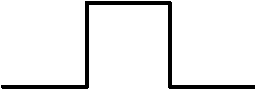
\includegraphics[scale=1]{IntSquare}
	} ~
	\subfloat[$F + F + + F - F - - F F - F$, turning angle: $60^{\circ}$]{
		\hspace{9mm}
\includegraphics[scale=1]{IntHexa}\hspace{9mm}
	}
	\caption{Examples of interpretation simple string of symbols}
	\label{fig:intSequences}
\end{figure}


More complex string of symbols as an example of interpretation is generated by \lsystem in \autoref{lsys:intExampleCode} where symbol $F$ is interpreted as \emph{draw line forward},
	symbol $+$ is interpreted as \emph{turn left} by 85 degrees and symbol $-$ as \emph{turn right} by 85 degrees (equally as \emph{turn left} by $-85$ degrees).
Result of interpretation of the first, second and fourth iteration is in \autoref{fig:intExample}.

\begin{Lsystem}[label=lsys:intExampleCode,caption={Symbol interpretation example}]
lsystem InterpretationExample {
	set symbols axiom = F;
	set iterations = 4;
	@interpret F as DrawForward(10);@
	@interpret + as TurnLeft(85);@
	@interpret - as TurnLeft(-85);@
	rewrite F to F + F - - F + F;
}
process all with SvgRenderer;
\end{Lsystem}

\begin{figure}[h]
	\subfloat{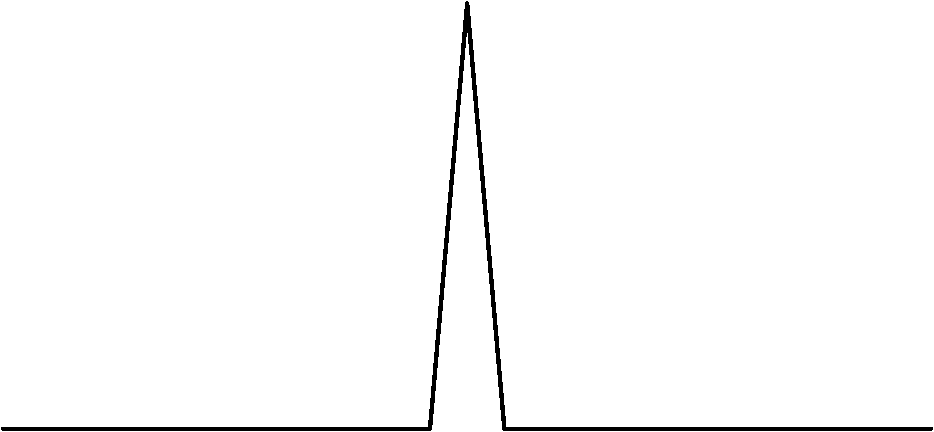
\includegraphics[scale=0.5]{Interpretation1}} \hfill
	\subfloat{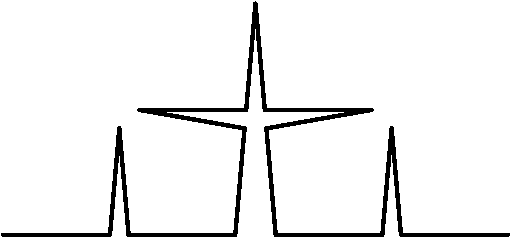
\includegraphics[scale=0.5]{Interpretation2}} \hfill
	\subfloat{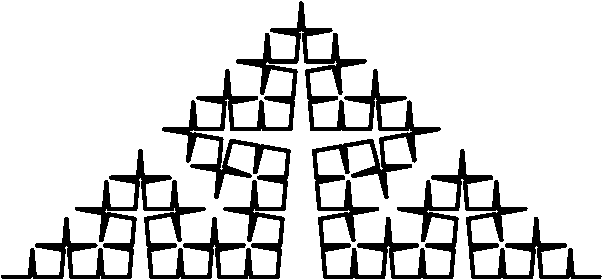
\includegraphics[scale=0.5]{Interpretation4}}
	\caption{The first, second and fourth iteration of the Cesaro curve (\autoref{lsys:intExampleCode})}
	\label{fig:intExample}
\end{figure}

\begin{figure}[h]
	
\includegraphics[width=1\linewidth]{RowOfTrees}
	\caption{Enhanced Cesaro curve from \autoref{fig:intExample} \cite[p.~48]{PL91}}
	\label{fig:rowOfTrees}
\end{figure}




































\clearpage

\section{\lsystem types}
\label{sec:lsysTypes}

In this section is described different types of \lsystems.
Some types may require an extension to the described formal definition of an \lsystem but this will be omitted here.

The \lsystems described so far are called \emph{deterministic \lsystems} because their rewriting system is deterministic.
\emph{Bracketed \lsystems} allow to save and load a state of the interpretation;
	this can be used to model branches of plants more easily.
\emph{Stochastic \lsystems} can randomize a result model to suppress its artificiality.
\emph{Context-sensitive \lsystems} allow to rewrite symbols depending on their context (the neighboring symbols around them).
Symbols in \emph{parametric \lsystems} can hold any number of arguments that can be used while rewriting or interpreting symbols.

Any of the above-described types can be combined together.



\subsection{Deterministic \lsystems}

\newcommand{\dzerolsystem}{\mbox{D0L-system}\xspace}
\newcommand{\dlsystem}{\mbox{dL-system}\xspace}


\begin{wrapfigure}{r}{0.50\textwidth}
	\vspace{-30pt}
	
\includegraphics[width=\linewidth]{BasicLsystem}
	\caption{Dragon curve}
	\label{fig:basicLsystem}
\end{wrapfigure}


The basic \lsystem type described by the previous formal definition is called a \dzerolsystem\footnote{A \dzerolsystem is also just called a \dlsystem~\cite{Zar04}.}.
\emph{D} means that the rewriting is deterministic and \emph{0} means it is context-free.
The result of a \dzerolsystem depends only on the initial string of symbols.

This type of \lsystem is often used to generate fractal curves.
With the \dzerolsystem in \autoref{fig:basicLsystem} we can generate the Dragon curve that you can see in \autoref{lsys:basicLsystemSrc}.

\begin{Lsystem}[label=lsys:basicLsystemSrc,caption={\dzerolsystem for the generation of the Dragon curve (\autoref{fig:basicLsystem})}]
lsystem DragonCurve {
	set iterations = 12;
	set symbols axiom = L;
	interpret R L as DrawForward(5);
	interpret + as TurnLeft(90);
	interpret - as TurnLeft(-90);
	rewrite L to L + R +;
	rewrite R to - L - R;
}
process all with SvgRenderer;
\end{Lsystem}


\subsection{Bracketed \lsystems}

A bracketed \lsystems\cite[p.~24]{PL91} extends basic \dzerolsystem with a branching system.
Branching is such a fundamental feature that Bracketed \lsystems are often just called \lsystems.

A branching system brings two new commands to the symbol interpretation system: \emph{start branch} and \emph{end branch}.
These commands are nearly always represented as bracket symbols (from which bracketed \lsystems got their name).
An open bracket "\texttt{[}" as a start branch and close bracket "\texttt{]}" as a close branch.

The start branch command saves the state of interpretation, which can then be loaded by end the branch command later.
In turtle graphics, the interpretation state is the position, orientation and drawing color of the turtle.
More than one state can be saved at the same time, and the last saved state will be loaded first.
This behavior seems natural and could be compared to a pairing of brackets.

Branching extends a linear string of symbols to a tree structure.
Individual branches do not affect each other nor their root.
This allows plants to be modeled more easily and to create more complex models.

The bracketed \lsystem in \autoref{lsys:branchingSrc} demonstrates a use of the branching system to produce a plant-like model as can be seen in \autoref{fig:branching}.
Note that the color of segments indicates their type and age.
Black segments are drawn with the symbol \texttt{F} and they represent segments from the previous iteration.
Green segments are drawn with the symbol \texttt{A} and they are new compared to the previous iteration.

\begin{Lsystem}[label=lsys:branchingSrc,caption={A bracketed \lsystem that which creates a plant-like model (\autoref{fig:branching})}]
lsystem PythagorasTree {
	set symbols axiom = A;
	set initialAngle = 90;
	set iterations = 4;	
	interpret A F as DrawForward(16);
	interpret + as TurnLeft(45);
	interpret - as TurnLeft(-45);
	@interpret [ as StartBranch;@
	@interpret ] as EndBranch;@
	rewrite A to F [ + A ] [ - A ] F A;
	rewrite F to F F;
}
process all with SvgRenderer;
\end{Lsystem}

\begin{figure}[h]
	\centering
	\subfloat{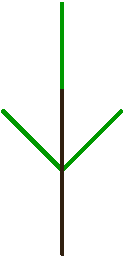
\includegraphics[scale=1]{Branching1}} ~
	\subfloat{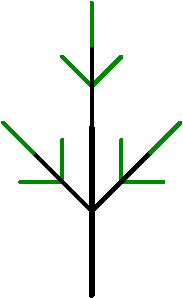
\includegraphics[scale=1]{Branching2}} ~
	\subfloat{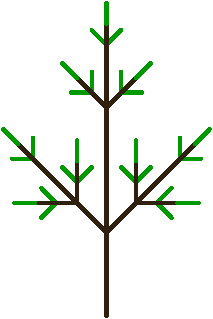
\includegraphics[scale=1]{Branching3}} ~
	\subfloat{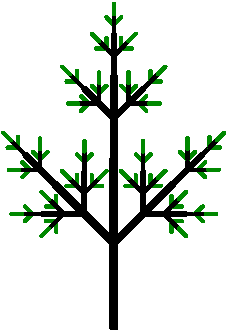
\includegraphics[scale=1]{Branching4}}
	\caption[The first four iterations of a bracketed \lsystem]{The first four iterations of the bracketed \lsystem in \autoref{lsys:branchingSrc}}
	\label{fig:branching}
\end{figure}



\subsection{Stochastic \lsystems}

\newcommand{\zerolsystem}{\mbox{0L-system}\xspace}
\newcommand{\zerolsystems}{\mbox{0L-systems}\xspace}

All plant models generated by the same deterministic \lsystem are identical.
However, a forest made by trees which are all identical looks artificial and can not be used in films or video games.
Stochastic \lsystems solve this problem because they can produce a randomized model.
Stochastic \lsystems are called \zerolsystem where 0 means they are context-free.

Randomization of a model produced by stochastic a \lsystem can be done in two places, in the rewrite rules or in the interpretation of symbols (or in both).
Randomization in interpretation can only change the properties of such interpreted symbols as lengths of lines or turning angles, while the topology of the model remains unchanged.
This is in contrast to rewrite rule randomization that can also change the topology of a model.
Rewrite rule randomization is achieved by defining more replacements for one rewrite rule.
The rewriting system will pick a random replacement if the rewrite rule is applied.
Each replacement can have a different probability of being picked.

In \autoref{fig:randComparison}, three models of a plant generated by stochastic \lsystems are shown.
The first image (\ref{fig:randComparisonNo}) was generated without any randomization.
The second image (\ref{fig:randComparisonInt}) was generated with interpretation randomization of line lengths and angles.
For the last image (\ref{fig:randComparisonBoth}) was used the rewrite rule randomization which changed the topology of the model (\autoref{lsys:randExample}).

\begin{figure}[h]
	\centering
	\subfloat[No randomization]{
		\label{fig:randComparisonNo}
		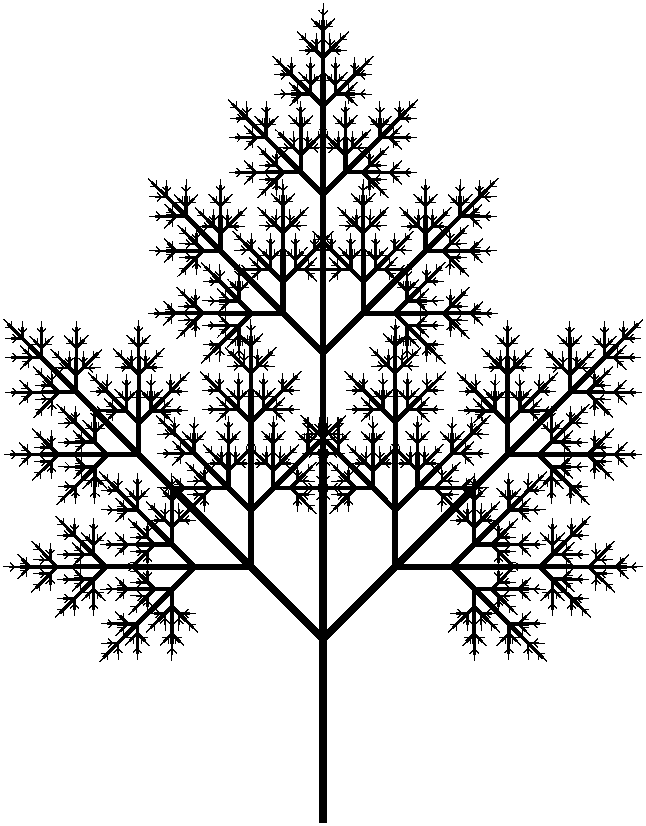
\includegraphics[width=0.3\textwidth]{StochasticLsystemExample-NoStochasism}
	} ~
	\subfloat[Angles, lengths randomized]{
		\label{fig:randComparisonInt}
		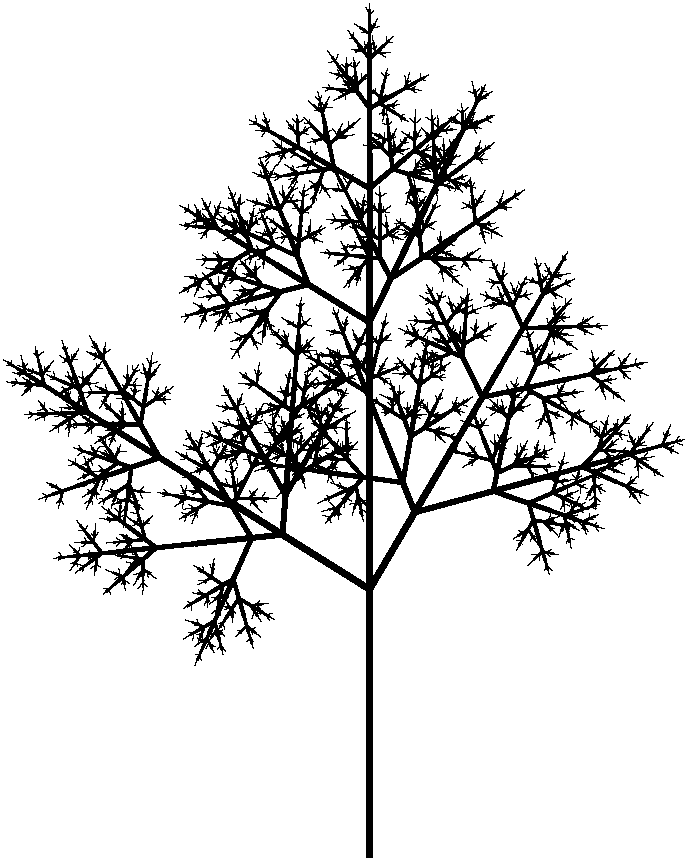
\includegraphics[width=0.32\textwidth]{StochasticLsystemExample-InterpretationStochasism}
	} ~
	\subfloat[Also topology randomized]{
		~
		\label{fig:randComparisonBoth}
		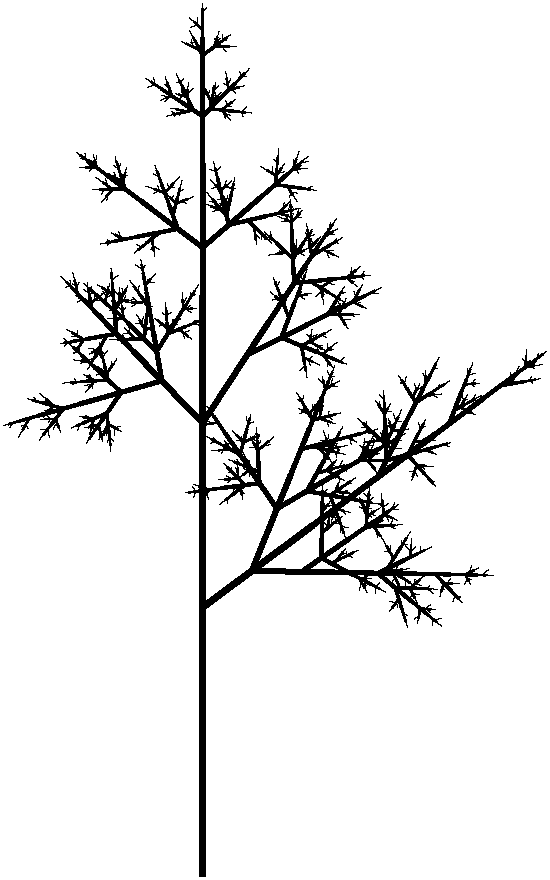
\includegraphics[width=0.25\textwidth]{StochasticLsystemExample-BothStochasism}
		~
	}
	\caption{A comparison between a non-randomized and randomized plant model}
	\label{fig:randComparison}
\end{figure}

\begin{Lsystem}[label=lsys:randExample,caption={Stochastic \lsystem with randomized interpretation of symbols and rewrite rule replacements}]
lsystem StochasticLsystemExample {
	set symbols axiom = X;
	set iterations = 8;
	set initialAngle = 90;
	interpret F(age) as DrawForward(@1.8^age*random(0.5,1.5)@, age/2);
	interpret + as TurnLeft(@45 + random(-20, 20)@);
	interpret - as TurnLeft(@-45 + random(-20, 20)@);
	interpret [ as StartBranch;
	interpret ] as EndBranch;
	rewrite F(age) to F(age + 1);
	@rewrite X@
		@to F(1) [ + X ] [ - X ] F(1) X  weight 4 or@
		@to F(1) [ + X ]         F(1) X  weight 1 or@
		@to F(1)         [ - X ] F(1) X  weight 1;@
}
process all with SvgRenderer;
\end{Lsystem}


\subsection{Context-sensitive \lsystems}

\newcommand{\onelsystems}{\mbox{1L-systems}\xspace}
\newcommand{\twolsystems}{\mbox{2L-systems}\xspace}

The rewriting of symbols in \zerolsystems is context-free; the rewrite rules are applied to the symbols regardless of their context (the symbols around them).
However, the rewriting of a symbol can also depend on its context.
This is useful in simulating the flow of signals (nutrients or hormones) in a plant model that, for example, attempts to demonstrate natural plant growth~\citep{PL91}.

Formally there are two types of context-sensitive L-systems, \onelsystems and \twolsystems.
The rewrite rules of \onelsystems checks the context only to one side (left or right), whereas the rewrite rules of \twolsystems checks the context on both sides.
Since \onelsystems are just \twolsystems with one context empty we will consider context-sensitive \lsystems as \twolsystems.

The context-sensitive \lsystem in \autoref{lsys:signalPropagarionSrc} shows a simulation of signal propagation in a string of symbols; the result is given in \autoref{fig:signalPropagarion}.

\begin{Lsystem}[label=lsys:signalPropagarionSrc,caption={Context-sensitive \lsystem simulating signal propagation}]
lsystem RewritingExample {
	set symbols axiom = B A A A A A;
	set iterations = 6;
	set interpretEveryIteration = true;
	@rewrite {B} A     to B;@
	@rewrite     B {A} to A;@
}
process all with SymbolPrinter;
\end{Lsystem}

\begin{table}[h]
	\centering
	\begin{tabular}{c l}
   		\toprule
   		Iteration & String of symbols \\
   		\midrule
		0 & B A A A A A \\
		1 & A B A A A A \\
		2 & A A B A A A \\
		3 & A A A B A A \\
		4 & A A A A B A \\
		5 & A A A A A B \\
		6 & A A A A A A \\
		\bottomrule
	\end{tabular}
	\caption{An axiom and the first 6 iterations of an \lsystem in \autoref{lsys:signalPropagarionSrc} showing signal propagation in the given string of symbols}
	\label{fig:signalPropagarion}
\end{table}


\subsubsection{Context-sensitive bracketed \lsystems}
\label{sec:bracketedLsystems}

If we add context-sensitive rewrite rules to bracketed \lsystems the situation becomes more difficult.
The context-matching procedure must take into account the branches.
The following rules define the natural behavior of context between branches:
\begin{enumerate*}
	\item \label{enum:ctxRule1} two symbols are neighbors even if there are some branches between them,
	\item \label{enum:ctxRule2} the left neighbor of the first symbol in a branch is a symbol before the branch,
	\item \label{enum:ctxRule3} the last symbol in a branch does not have a right neighbor,
	\item \label{enum:ctxRule4} unmatched symbols at the end of a branch are ignored,
	\item \label{enum:ctxRule5} the order of branches is insignificant.
\end{enumerate*}

In \autoref{tbl:bracketCtxt} is a few examples of how a symbol with its context will match (or not) a given string of symbols with respect to the context-matching rules mentioned above.
\begin{table}[h]
	\centering
	\begin{tabular}{c c c | p{128pt} c c}
   		\toprule
   		Left ctx. & Symbol & Right ctx. & Symbol string & Match & Rule\\
   		\midrule
		 & X & Y & A B {\btHL\bf X} [ A [ B ] ] [ C ] {\btHL\bf Y} & yes & \ref{enum:ctxRule1} \\
		 & X & Y & A B X [ Y B ] C Y & no &  \\
		 Y & X & & A B {\btHL\bf Y [ X} A B ] C & yes & \ref{enum:ctxRule2} \\
		 Y & X & & A B {\btHL\bf Y [ [ X} A ] B ] C & yes & \ref{enum:ctxRule2} \\
		 & X & Y & A [ B X ] Y & no & \ref{enum:ctxRule3} \\
		 & X & [ Y ] & A B {\btHL\bf X [ Y} A B ] A  & yes & \ref{enum:ctxRule4} \\
		 & X & [ [ Y ] ] & A B {\btHL\bf X [ [ Y} A B ] C ] & yes & \ref{enum:ctxRule4} \\
		 & X & [ Y ] & A B {\btHL\bf X} [ A B ] {\btHL\bf{}[ Y} ] A  & yes & \ref{enum:ctxRule5} \\
		 & X & [ Y ] [ Z ] & A B {\btHL\bf X [ Z} ] {\btHL\bf{}[ Y} ] A  & yes & \ref{enum:ctxRule5} \\
		\bottomrule
	\end{tabular}
	\caption{Examples of context matching in bracketed \lsystems}
	\label{tbl:bracketCtxt}
\end{table}

Context in bracketed \lsystems can be used for the propagation of signals through tree structures.
There are two basic types of signals: the first is the \emph{acropetal} signal which spreads from the root to branches; and the second signal is \emph{basipetal} which spreads in the opposite way i.e. from branches to root.
This can be very useful in plant modeling.

\autoref{fig:signalPropagation} shows a simulation of acropetal (\ref{fig:acropetalSignal}) and basipetal (\ref{fig:basipetalSignal}) signals in a static plant-like structure.
Each figure shows the first 5 iterations and segments with the signal marked as a bolder line.
The \lsystem in \autoref{lsys:signalPropagation} simulates acropetal signal propagation and its result is in \autoref{fig:acropetalSignal} (image) and \autoref{fig:signalPropagationTable} (symbols).

\begin{figure}[h!]
	\centering
	\subfloat[Acropetal signal propagation]{
		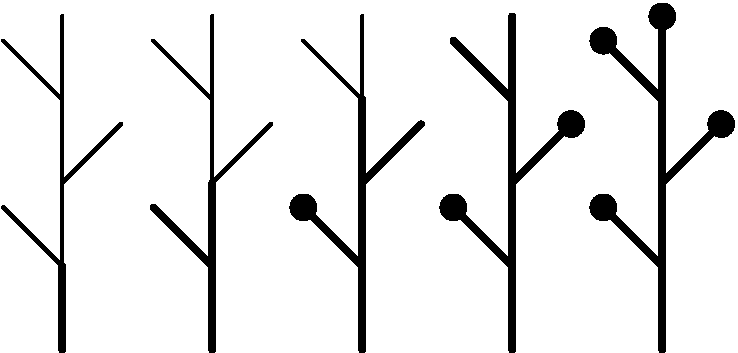
\includegraphics[scale=0.55]{AcropetalSignal}
		\label{fig:acropetalSignal}
	}
	\hspace{2mm}
	\subfloat[Basipetal signal propagation]{
		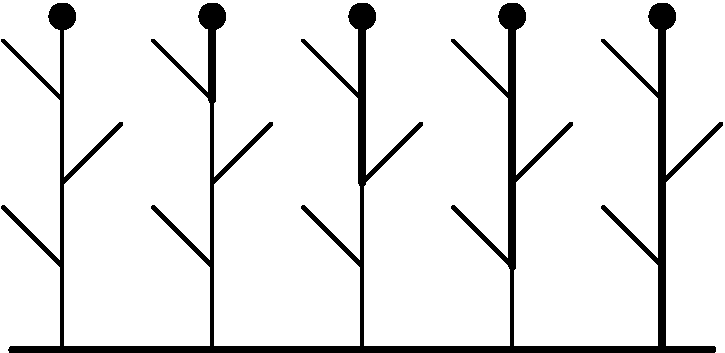
\includegraphics[scale=0.55]{BasipetalSignal}
		\label{fig:basipetalSignal}
	}
	\caption{Signal propagation simulated with context-sensitive bracketed \lsystems}
	\label{fig:signalPropagation}
\end{figure}

\begin{Lsystem}[label=lsys:signalPropagation,caption={The \lsystem simulating acropetal signal propagation (\autoref{fig:acropetalSignal})}]
lsystem AcropetalSignal extends Branches {
	set symbols axiom = B [ + A ] A [ - A ] A [ + A ] A;
	// ignore + and - symbols in context search
	@set symbols contextIgnore = + -;@
	set iterations = 3;
	// interpret every iteration to see signal propagation
	set interpretEveryIteration = true;
	set initialAngle = 90;
	interpret A as DrawForward(50, 2);
	interpret B as DrawForward(50, 4);
	interpret + as TurnLeft(45);
	interpret - as TurnLeft(-45);
	@rewrite { B } A to B;@
}
process all with SvgRenderer;
\end{Lsystem}


\begin{table}[h]
	\centering
	\begin{tabular}{c c}
   		\toprule
   		Iteration & String of symbols \\
   		\midrule
		0 & B [ + A ] A [ - A ] A [ + A ] A \\
		1 & B [ + B ] B [ - A ] A [ + A ] A \\
		2 & B [ + B ] B [ - B ] B [ + A ] A \\
		3 & B [ + B ] B [ - B ] B [ + B ] B \\
		\bottomrule
	\end{tabular}
	\caption{The result of the \lsystem simulating acropetal signal propagation in \autoref{lsys:signalPropagation}}
	\label{fig:signalPropagationTable}
\end{table}


\subsection{Parametric \lsystems}

Symbols in parametric \lsystems can hold any number of arguments.
Arguments are often floating point numbers, but they can be much more complicated structures.
Arguments can be used in interpretation definition to send values like color or length of line to an interpretation routine.
Arguments can also be used in rewrite rules to determine whether to rewrite a symbol or not, and to determine new arguments for rewritten symbols.
In context \twolsystems it is also possible to get arguments from symbols in context and use them in rewrite rules.

The \lsystem in \autoref{fig:scParams} shows an example of how the parameters of symbols can be used in interpretation methods and in rewrite rules together with the result.

\newsavebox{\lstBox}
\begin{lrbox}{\lstBox}
\begin{Lsystem50}
lsystem Circles {
	set symbols axiom =	[ X ] +
		[ X ] + [ X ] + [ X ];
	set iterations = 7;
	interpret F as MoveForward;
	interpret K as DrawCircle;
	interpret + as @TurnLeft(90)@;
	interpret - as @TurnLeft(-90)@;
	interpret [ as StartBranch;
	interpret ] as EndBranch;
	rewrite @K(n) to K(2*n)@;
	rewrite @F(n) to F(2*n)@;
	rewrite X to @K(2) F(3)@
		[ + X ] [ - X ] X;
}
process all with SvgRenderer;
\end{Lsystem50}
\end{lrbox}

\begin{figure}[h!]
	\subfloat{
		\usebox{\lstBox}
	} \hfill
	\subfloat{
		\minipage{0.47\linewidth}\noindent
		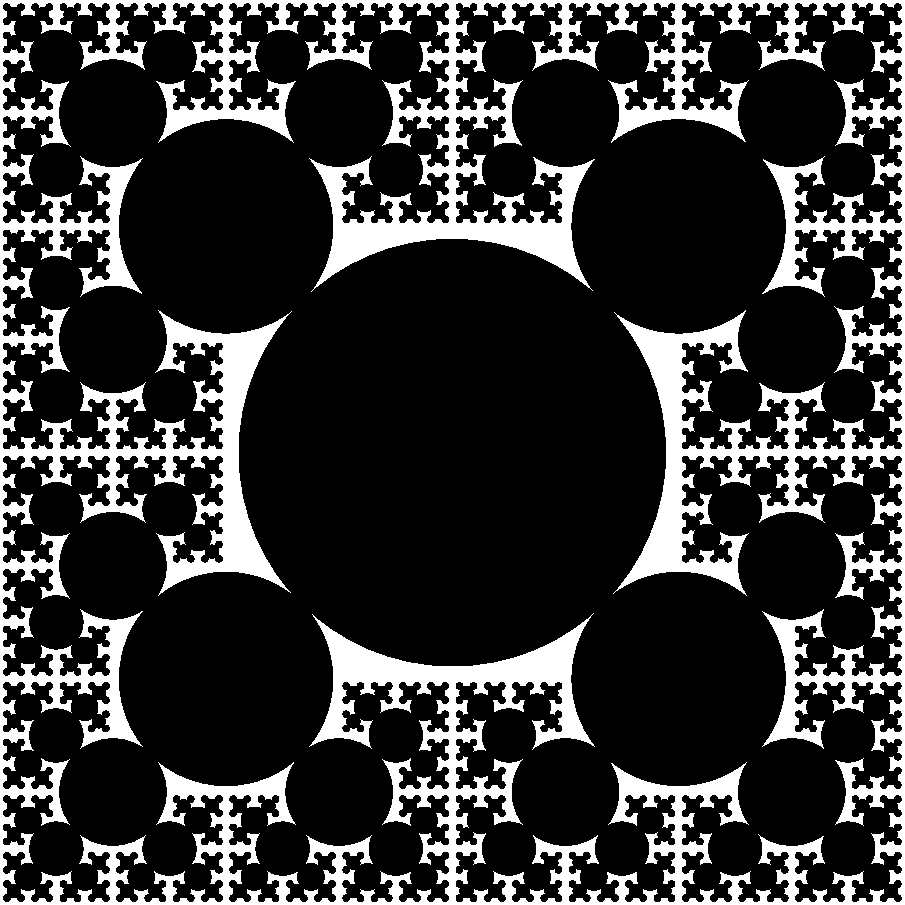
\includegraphics[width=\textwidth]{Circles}
		\endminipage
	}
	\caption{Parameters usage in \lsystem interpretation methods and in rewrite rules along with the result}
	\label{fig:scParams}
\end{figure}

In \autoref{fig:redEndPythagoras} is more complicated model, the Pythagoras tree.
Detailed instructions for its construction with \lsystems are described in appendix \ref{chap:userDoc}.

\begin{figure}[H]
	\centering
	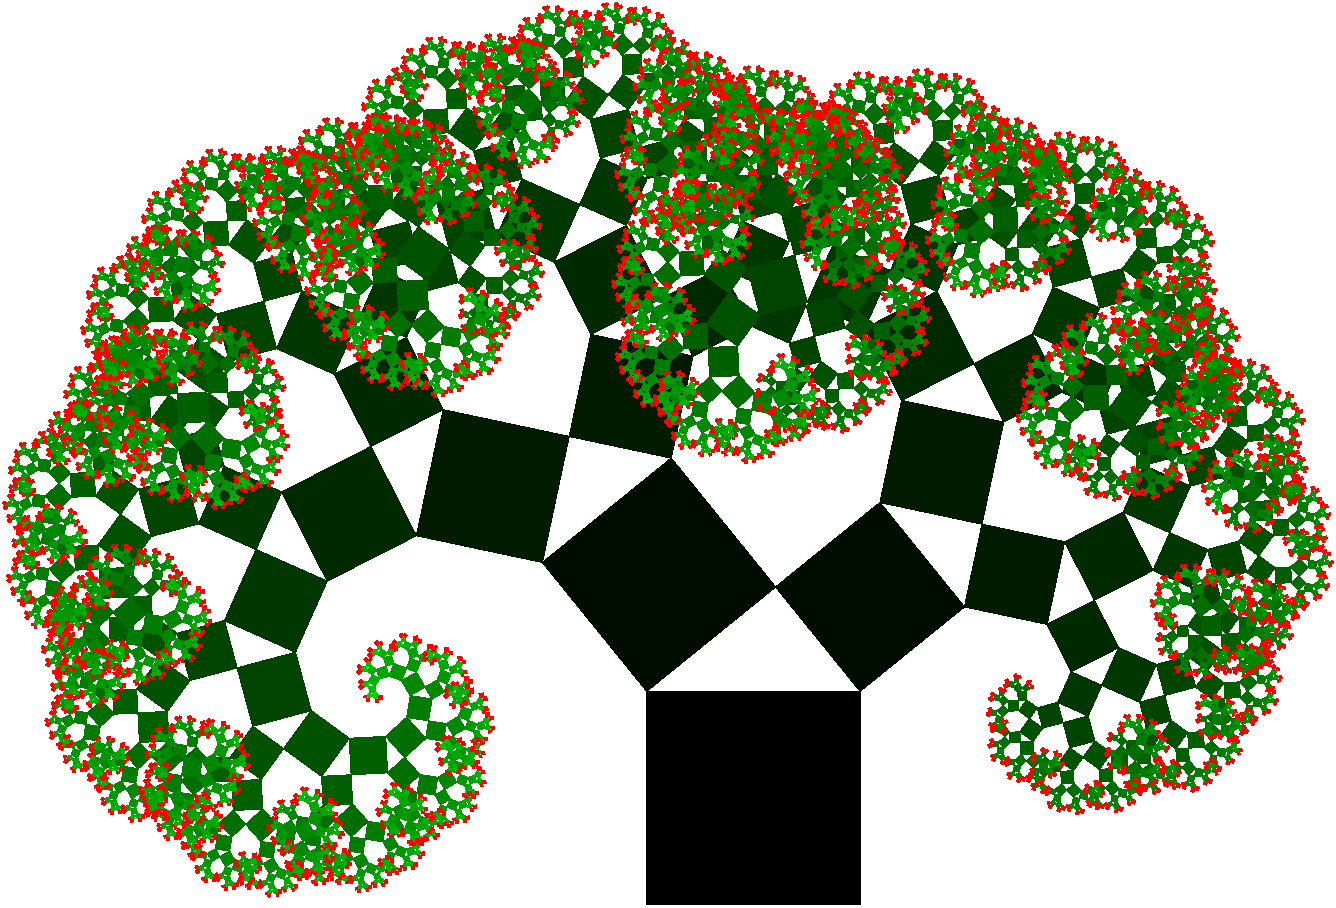
\includegraphics[width=\linewidth]{PythagorasTree2dRedEnd}
	\caption{Pythagoras tree created with parametric \lsystem}
	\label{fig:redEndPythagoras}
\end{figure}


































\clearpage

\section{Related \lsystem generators}

In this section are listed other computer programs or web pages that allow to process \lsystems and eventually interpret them in most cases as an image.

\subsection{Web based}
\label{sec:WebBasedGenerators}

\subsubsection{\lsystem generator by Michael Norris}
\srcurl{http://www.michaelnorris.info/software/l-system-generator.html}

\noindent
Simple script which allows to set basic properties of \lsystem namely number of iterations, axiom and up to 15 rewrite rules.
Result is a list of strings of symbols from all iterations (it does not interpret symbols).

This site can be used to familiarize with rewriting principles of \lsystems but it offers no additional functionality.


\subsubsection{Lindenmayer power by MadFlame Software}
\srcurl{http://madflame991.blogspot.com/p/lindenmayer-power.html}

\noindent
\lsystem generator which allows to set basic properties of \lsystem and interpretation for each symbol.
Symbols can be interpreted using turtle graphics or they can define or modify value of a variable.
All iterations are listed as text and drawn on screen as well.

Possibility to work with variables makes it relatively powerful system but it is possible to draw only with a thin black line.
Also the syntax is not very user-friendly and user the interface is hard to use (and the script it is not very stable).
The size of the output window is only $500 \times 500$ pixels and output can not be saved otherwise than using print-screen.


\subsubsection{\lsystem generator by Nolan Carroll}	
\srcurl{http://nolandc.com/sandbox/fractals/}

\noindent
\lsystem generator with a nice looking interface where it is possible to set basic properties of an \lsystem.
The interpretation of symbols is fixed.
Last iteration of \lsystem is drawn on the screen using animation (line by line from the starting position).

Interface is user friendly but only drawable interpretation of symbol is black line.
There is no help nor examples thus it is hard to use for inexperienced user.
Output is drawn on canvas which fills entire area of web browser but it can not be saved otherwise than using print-screen.


\subsubsection{VRML \lsystem generator by Patrick Murris}
\srcurl{http://www.alpix.com/vrml/lsys.htm}
  
\noindent
\lsystem generator which can generate 3D VRML model.
Basic properties of \lsystem and interpretation can be set and output can be produced into VRML 1.0, 2.0 or string.

The problem is that VRML plugin is needed for displaying 3D models.



\subsubsection{\lsystem generator by John Snyders}
\srcurl{http://hardlikesoftware.com/projects/lsystem/lsystem.html}

\noindent
At first sight it is sophisticated \lsystem generator which can rewrite symbols with parameters and do context-sensitive rewriting.
Result is drawn on a page as an animation of development and a progress bar shows its status.
The biggest drawback is that \lsystems are hard-coded in JavaScript and it is only possible to change the number of iterations.

This \lsystem generator contains many examples and output is rendered as image which can be saved but examples are the only thing what it can produce.


\subsubsection{WWW \lsystem Explorer by Zdík Kudrle}
\srcurl{http://zdeeck.borg.cz/wlse/l-system.php}

\begin{wrapfigure}{r}{0.45\textwidth}
	\vspace{-20pt}
	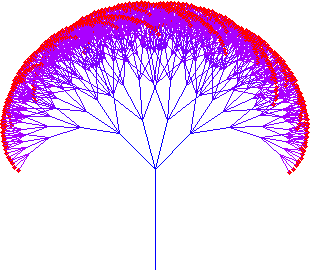
\includegraphics[width=\linewidth]{WwwLsystemExplorer}
	\caption{Image produced by WWW \lsystem Explorer}
	\label{fig:lsysExplorer}
\end{wrapfigure}

\noindent
\lsystem generator with well-arranged user interface where is possible to set basic properties of the generated \lsystems.
The interpretation of symbols is fixed and it uses unusual set of interpretation methods like \emph{pen up} and \emph{pen down} instead o traditional \emph{draw line} and \emph{move forward}.
The last iteration is drawn as an image by server-side PHP script thus output can be downloaded easily.
It is possible to set line color (even to color gradient) and background color of the image.
Size of the output image can be set freely.

This web-based generator is the best among the generators listed in this section.
It contains well written help section and a few examples.
However it can not do context rewriting and symbols can't hold any parameters.
The length of drawn lines or turns can be affected only by increasing \emph{depth level} and setting the change ratio.
Example of plantlike model produced by WWW \lsystem Explorer is in \autoref{fig:lsysExplorer}.




\subsection{Desktop applications}
\label{sec:DesktopGenerators}

\subsubsection{\lsystems explorer by James Matthews}
\label{sec:LsystemExplorer}
\srcurl{http://www.generation5.org/content/2002/lse.asp}

\noindent
Simple desktop application which renders \lsystems in the application window.
Basic properties of \lsystem and its interpretation can be edited in dialog window but interpretation for individual symbols can not be changed.
It is possible to move and zoom the model with a mouse.
\lsystems can be saved or loaded into text file and drawn image can be saved to clipboard.

\lsystems explorer can be used for generation of simple models but it is not possible to do context rewriting or use symbols parameters.
Even line thickness can not be changed.
User interface for editing \lsystem is very simple (it is possible to show rewrite rules only for one symbol at a time).


\subsubsection{\lsystem Vector Generator by Dmitry Malutin}
\srcurl{http://xaraxtv.at.tut.by/lsvg.htm}

\begin{wrapfigure}{r}{0.4\textwidth}
	\vspace{-20pt}
	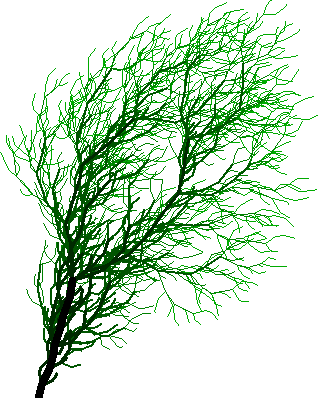
\includegraphics[width=\linewidth]{LsystemVectorGenerator}
	\caption{Plant example from \lsystem Vector Generator}
	\label{fig:lsvg}
\end{wrapfigure}

\noindent
Similar application to the \nameref{sec:LsystemExplorer} but with better user interface and it is also possible to randomize line lengths or turn angles.
Nice feature is the \emph{angle wizard} which displays grid of \lsystems each with different setting of turning angle and you can pick what you like. %!!!!!!!!!!!
Drawn lines can be automatically closed to form polygons.
It is possible to save image as AI (Adobe Illustrator) or WMF (Windows Metafile) file which are not very common formats.

Application contains hundreds of examples but it lacks any advanced types of \lsystems or interpretation settings.
Application window size is about $700 \times 550$ pixels and it can not be resided.
One of built-in examples with randomized angles and line lengths is in \autoref{fig:lsvg}.


\subsubsection{\lsystem 4 by Timothy Perz}
\srcurl{http://www.oocities.org/tperz/L4About.htm}

\noindent
\lsystem 4 is relatively advanced tool for generating models with \lsystems.
Besides all basic functionality it is possible to create 3D models with custom textures.
Models can be saved as raster images (BMP or JPEG) or they can be exported to AutoCAD DXF format.
Interpreting capabilities are quite good but it can do only deterministic rewriting with limited usage of parameters.

Table of symbols interpretations (which are not changeable) can be displayed at right side of application which is a nice feature.
\lsystem 4 has good capabilities in producing of 3D output but the input syntax is very compact and hard to read.
Also more advanced \lsystem types like context-sensitive or parametric \lsystems are not supported.

\newcommand{\lstudio}{\mbox{L-studio}\xspace}

\subsubsection{\lstudio by Przemysław Prusinkiewicz et. al}
\srcurl{http://algorithmicbotany.org/lstudio/}

\noindent
\lstudio is probably one of the best applications designed for modeling plants with \lsystems.
\lstudio is not a single program but it is complex solution that consists of many tools.
\lstudio can process all types of \lsystems described in \autoref{sec:lsysTypes} and also it can produce animation of plant growth.
With \lstudio is possible to model 3D models of plants with regards to environment like wind, gravity, the space around plant, sunlight, etc.
Output model can be saved in many formats like Wavefront OBJ, Postscript, BMP or it can be rendered with built in ray-tracer to produce photo-realistic images.

Even there is many examples of plant models and extensive help it is not easy to start using it.
The syntax is very compact and quite unclear for a new user.

Application is not free-ware but a demo version can be downloaded.
After evaluation period it is still possible to use it but it is not possible to export images and the previews have watermark.
In \autoref{fig:lstudio} is one of the most beautiful examples in \lstudio, the Lily.


\begin{figure}[h]
	\centering
	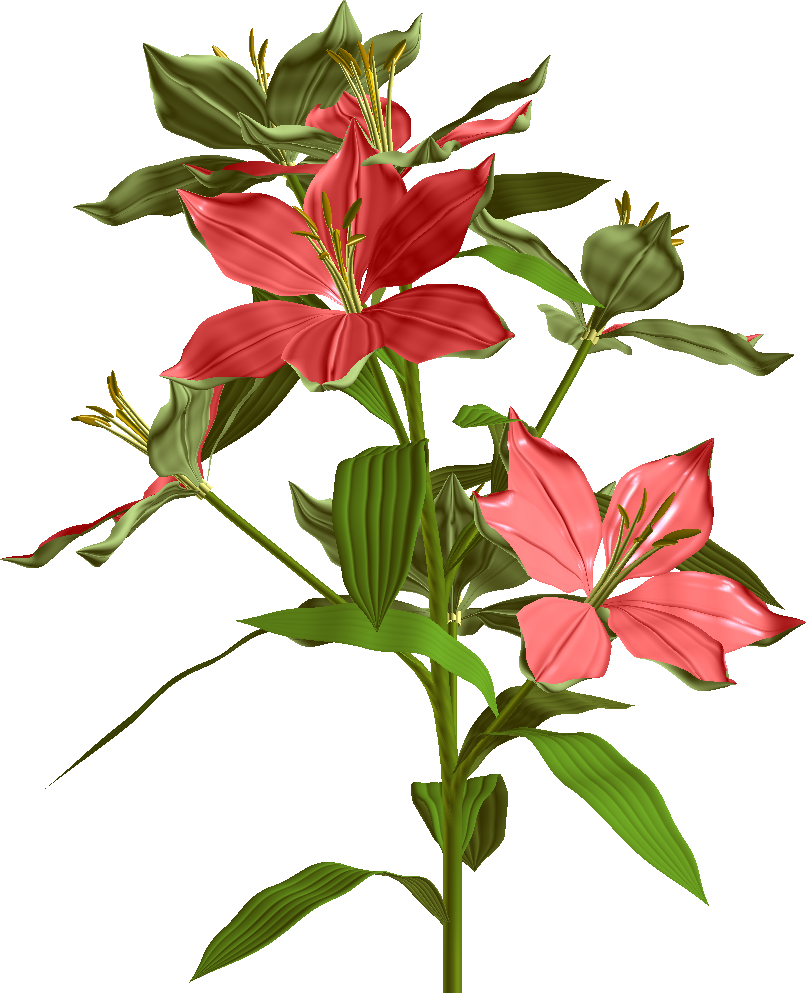
\includegraphics[width=0.8\linewidth]{Lily}
	\caption{Model of Lily produced by \lstudio}
	\label{fig:lstudio}
\end{figure}


























































\singlespacing
\nocite{*}  % Show all Bib-entries
\printbibliography

%\chapwithtoc{List of Figures}
%\listoffigures

%\chapwithtoc{Attachments}

\openright
\end{document}
